%%%%%%%%%%%%%%%%%%%%%%%%%%%%%%%%%%%%%%%%%
% Journal Article
% LaTeX Template
% Version 2.0 (February 7, 2023)
%
% This template originates from:
% https://www.LaTeXTemplates.com
%
% Author:
% Vel (vel@latextemplates.com)
%
% License:
% CC BY-NC-SA 4.0 (https://creativecommons.org/licenses/by-nc-sa/4.0/)
%
% NOTE: The bibliography needs to be compiled using the biber engine.
%
%%%%%%%%%%%%%%%%%%%%%%%%%%%%%%%%%%%%%%%%%

\documentclass[
	a4paper,         % Paper size: a4paper or letterpaper
	12pt,            % Default font size
	unnumberedsections,  % Comment to enable section numbering
	twoside,         % Two-side layout
]{LTJournalArticle}
\usepackage{amsmath}
\usepackage{booktabs}   % For professional looking tables
\usepackage{siunitx}    % Optional, for numeric alignment
\usepackage{graphicx}   % For \resizebox
\DeclareMathSizes{10}{10}{8}{7}
\addbibresource{reference.bib}

\runninghead{Monte Carlo Simulation of CDO Pricing - Mackenzie Qu}
\setcounter{page}{1}
\title{
Monte Carlo CDO Pricing and Correlation Impact
}

\date{Mackenzie Qu} % Date left empty
% Full-width abstract (left empty)
\renewcommand{\maketitlehookd}{%
	\begin{abstract}
    We develop and implement a hybrid Monte Carlo framework to price a five-year, four-tranche CDO on a high-yield North American CDX index.  Public issuers’ pairwise correlations are calibrated from weekly equity returns via a one-factor Gaussian-copula/CAPM model; private issuers and cross-pairs rely on Basel II/III IRB one-year PD–driven correlation floors.  CDS-implied default intensities are bootstrapped from 5-year spreads under a flat-hazard assumption (recovery = 40 \%).  Simulating $10^5$ default-time paths, we obtain fair spreads of 90 bp, 11 bp, 1.3 bp, and 0.015 bp for the 0–5 \%, 5–15 \%, 15–25\%, and 25–100 \% tranches respectively (SE < 1 bp).  A 10 \% uniform correlation bump reveals steep equity-tranche leverage ($\Delta$ 90 bp), modest mezzanine sensitivity ($\Delta$3 bp), and near-flat senior/super-senior behavior. 

	\end{abstract}
	\vspace{1ex}
}

\begin{document}
\maketitle
\section{Introduction}
Collateralized Debt Obligations (CDOs) allocate portfolio credit risk into tranches whose fair coupons depend crucially on joint default dynamics.  While the one-factor Gaussian copula (Li 2000) permits empirical calibration via equity return correlations, many CDO pools also include private or delisted names lacking market data.  Concurrently, Basel II/III’s Internal Ratings-Based (IRB) approach mandates conservative asset-correlation floors—12 \%–24 \%—anchored to one-year PDs.  We propose a hybrid methodology that seamlessly merges (1) historical, CAPM-beta-derived correlations for public firms, (2) PD-driven Basel IRB floors for private issuers, and (3) a flat-hazard mapping from 5-year CDS spreads to default intensities.  This enables a unified Monte Carlo simulation of default times and tranche cash flows, yielding fair spreads and sensitivities to correlation stress.


%----- Create three subsections corresponding to the three prompts in the IAQF Student Problem 2025 -----
\section{Methodology}
\subsection{Data Preparation} The constituent tickers and 5-year CDS spreads are sourced from a High-Yield CDX index, filtering out missing values for CDS spreads. Historical weekly closing prices (2010–2024) for public firms and SPY as benchmark are downloaded via Yahoo Finance\cite{yfinance}; private tickers lacking equity data are mapped to the Basel IRB framework\cite{bcbs_irb_2005}.

To separate the public traded companies and the private companies, we operated 2 rounds of yfinance download. The tickers that did not retrieve historical data in the first round were individually searched and are identified as: 
\begin{enumerate}
    \item Alternative Ticker Format
    \item Subsidiary of Publicly Traded Parent Company
    \item Merger and Acquisition
    \item Privately Traded Company
\end{enumerate}

A second round of downloads was performed, and the tickers that failed to download were appended to the public company list. 

As a result, the finally private companies were identified as below in Table\ref{tab:private}.

\begin{table}[h!]
\centering
\resizebox{\linewidth}{!}{%
\begin{tabular}{|l|r|}
\hline
\textbf{Company Name} & \textbf{CDS Spread (bps)} \\
\hline
Ashland Inc & 78.94 \\
CSC Holdings LLC & 139.45 \\
DISH DBS Corp & 3268.47 \\
Domtar Corp & 78.94 \\
EQM Midstream Partners LP & 221.16 \\
Liberty Interactive LLC & 2309.78 \\
NOVA Chemicals Corp & 357.72 \\
RR Donnelley \& Sons Co & 121.90 \\
Rite Aid Corp & 4250.82 \\
Staples Inc & 1773.46 \\
ADT Security Corp/The & 118.36 \\
Gap Inc/The & 188.22 \\
Hertz Corp/The & 430.18 \\
Vistra Operations Co LLC & 137.33 \\
\hline
\end{tabular}%
}
\caption{CDS Spreads for Selected Companies}
\label{tab:private}
\end{table}

\subsection{Default Probability Extraction}Under a flat-hazard assumption, a CDS spread S implies hazard $\lambda = S/(1-R)$ and a cumulative one-year PD
$PD_1 = 1 - e^{-\lambda\cdot1}$\cite{hull_derivatives_2022}. Based on Moody's recovery rate of 38\%\cite{moodys_ultimate_recovery_database} and SP Global\cite{spglobal_loan_recoveries_2023} recovery rate of 44\%, we estimated a recovery rate R=40\% as the market average for senior unsecured bonds. This yields a uniformly calibrated PD vector for all names.

\subsection{Basel II/III IRB Asset Correlations}
For each issuer’s one-year PD, the IRB formula defines asset correlation
$$\rho_i=0.12\frac{1 - e^{-50\,PD_i}}{1 - e^{-50}}
+0.24\Bigl(1 - \frac{1 - e^{-50\,PD_i}}{1 - e^{-50}}\Bigr)$$,
ensuring $\rho_i\in[0.12,0.24]$. Pairwise correlations follow $\rho_{ij}=\sqrt{\rho_i\,\rho_j}$

This gives a full $N\times N$ correlation matrix where:
\begin{itemize}
    \item Diagonal entries $\rho_{ii}=1$ by construction
    \item Off-diagonals lie in $[0.12,\,0.24]$
\end{itemize}

In our High Yield CDX universe, applying this methodology to each issuer’s one-year PD (bootstrapped from its 5-year CDS spread) yields a minimum pairwise correlation of 0.1200 - occurs between two very high‐PD names whose individual $\rho_i$ values both sit at the regulatory minimum of 12 \%, and a maximum pairwise correlation of 0.2077 - arises between two of the lowest‐PD names.

These bounds reflect the regulatory intent: to impose a conservative baseline correlation for capital calculation, independent of empirical co-movement measures.

\subsection{CAPM-Based Equity Correlation}
For each public firm, we compute weekly log-returns and estimate CAPM betas via OLS against the SPY ETF. 
$$r_{i,t} \;=\;\alpha_i \;+\;\beta_i\,r_{M,t}\;+\;\epsilon_{i,t}$$,
where $r_{M,t}$ are SPY log-returns.  The estimated slope $\beta_i$ measures firm i’s systematic exposure to the market factor.

Under CAPM, total variance of $r_{i}$ splits into a systematic component $\beta_i^2 Var(r_M)$ and an idiosyncratic component $Var(\epsilon_i)$.  We estimate

$$\widehat{Var}(\epsilon_i)
= \widehat{Var}(r_i) \;-\; \beta_i^2\,\widehat{Var}(r_M)$$

ensuring no negative idiosyncratic variance via truncation at zero.

Applying this procedure to the public names yields a minimum pairwise correlation of 0.0458 and a maximum of 0.4955, reflecting the broad diversity of how different firms’ equity returns have co-moved with the market and each other over the 2010–2024 period.

\subsection{Monte Carlo CDO Pricing}

To simulate one-factor Gaussian Copula for default dependence, we first sample from correlated normal distribution and transform it into uniforms. Assuming default events follows an exponential distribution, we can inverse the exponential mapping with the hazard rate derived from the CDS Spread. 

With each tranche exposure change only at default times, we identify the default times that fall before maturity and accrue the premium leg over each interval and allocate default-leg losses at each default time by updating the tranche loss fraction.

For each Monte Carlo scenario i, we compute
$$q_i = \frac{\text{PV of default‐leg losses}}
{\text{PV of premium leg accruals}}
\;\approx\;\frac{\sum_m\Delta\text{Loss}_m}{\sum_m \text{Out}_m \cdot \Delta t_m}$$

The break-even coupon q per tranche is the ratio of expected default losses to premium accrual, replicated across four tranches: equity (0–5 \%), mezzanine (5–15 \%), senior (15–25 \%), and super-senior (25–100 \%)



\section{Results}
With the combined correlation matrix for both public and private firms, the Monte Carlo simulation provided the following results for the fair spread of each tranche in Table \ref{tab:fair_spreads}.

As the first‐loss position, the Equity tranche is most sensitive to the expected portfolio loss over five years. A nearly 1\% coupon compensates for the roughly 5\% attachment point combined with moderate default probabilities (average CDS‐implied intensities ~0.058 \%) and our hybrid correlations (average of 22.38 \%).

\begin{table}[h!]
\centering
\resizebox{\linewidth}{!}{
\begin{tabular}{c c c c c}
\hline
\textbf{Tranche} & \textbf{Attach} & \textbf{Detach} & \textbf{Fair Spread} & \textbf{Std. Err.} \\
\hline
Equity & 0.00 & 0.05 & 0.899598 & 0.006893 \\
Mezzanine & 0.05 & 0.15 & 0.109642 & 0.000781 \\
Senior & 0.15 & 0.25 & 0.012656 & 0.000213 \\
Super Senior & 0.25 & 1.00 & 0.000148 & 0.000006 \\
\hline
\end{tabular}
}
\caption{Fair spreads and standard errors by tranche}
\label{tab:fair_spreads}
\end{table}

Protected by the equity cushion, the Mezzanine tranche’s spread falls an order of magnitude to ~0.11 \%. It primarily reflects the probability that portfolio losses exceed 5 \% but stay below 15\%, a lower‐frequency event.

Only extreme default clusters breach the 15\% attachment, so senior spreads collapse to ~1 bp, and the coupon for the Super Senior tranche is nearly zero.

\subsection{Tranche sensitivity to correlation}
To investigate the tranche sensitivity to correlations among issuers, we implemented a change in correlation from -0.05 to 0.05. we added $\Delta\rho$ to every off-diagonal element of the combined correlation matrix and re-priced all four tranches via Monte Carlo.

Figure \ref{fig:corr_bump} shows how each tranche's fair spread responds to the uniform bumps in the underlying default-correlation matrix.

We can observe the equity slice exhibits by far the greatest sensitivity, with its fair spread rising from approximately 83 bp at a –10 \% correlation change to about 102 bp at +10 \%.  This steep slope reflects that higher correlations concentrate losses into fewer, more extreme scenarios, thereby heightening the risk borne by the first‐loss bucket.

The mezzanine tranche’s spread increases modestly, from 10 bp to 12 bp. This intermediate sensitivity is consistent with its position in the capital structure: it absorbs losses only after the equity bucket is exhausted, so it is less exposed to increases in tail‐risk clustering .

Senior climbs from ~0.5 bp to ~2.2 bp, illustrating that even deep-loss buckets respond measurably when correlations are stressed by two standard deviations, which Super-Senior remains virtually flat at sub-basis-point levels, though it doubles its spread in percentage terms.


\begin{figure}[ht]
  \centering
  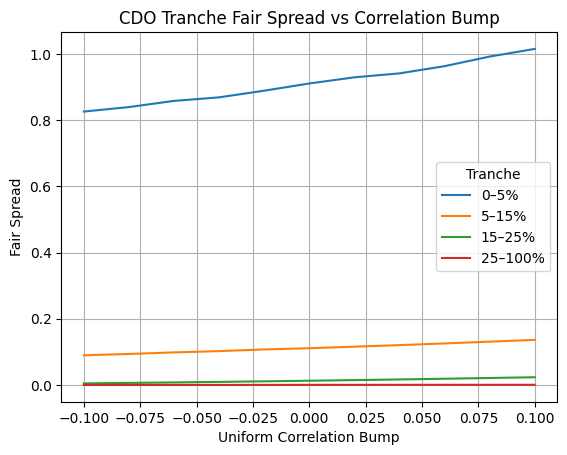
\includegraphics[width=0.5\textwidth]{Figures/output.png}
  \caption{Sensitivity of CDO tranche fair spreads to uniform correlation bumps of $\pm10\%$.}
  \label{fig:corr_bump}

\end{figure}

\begin{table}[ht]

  \centering
  \caption{Tranche Fair Spreads under Uniform Correlation Bumps}
  \label{tab:corr_bump_values}
  \resizebox{\linewidth}{!}{
  \begin{tabular}{rrrrr}
    \toprule
    \(\Delta\rho\) & 0–5 \% & 5–15 \% & 15–25 \% & 25–100 \% \\
    \midrule
    -0.10 & 0.826326 & 0.089636 & 0.004662 & 0.000014 \\
    -0.08 & 0.839838 & 0.093571 & 0.006083 & 0.000027 \\
    -0.06 & 0.858525 & 0.098284 & 0.007599 & 0.000045 \\
    -0.04 & 0.869260 & 0.102254 & 0.009143 & 0.000071 \\
    -0.02 & 0.889383 & 0.107280 & 0.010893 & 0.000104 \\
     0.00 & 0.911161 & 0.110945 & 0.012695 & 0.000144 \\
     0.02 & 0.929794 & 0.115658 & 0.014540 & 0.000193 \\
     0.04 & 0.941734 & 0.120282 & 0.016539 & 0.000244 \\
     0.06 & 0.963475 & 0.125448 & 0.018689 & 0.000297 \\
     0.08 & 0.992532 & 0.130737 & 0.020985 & 0.000356 \\
     0.10 & 1.015636 & 0.136185 & 0.023250 & 0.000428 \\
    \bottomrule
  \end{tabular}
  }
\end{table}

\section{Limitations}

While our hybrid framework effectively integrates empirical equity correlations for public issuers with conservative Basel II/III–driven floors for private names, it relies on several simplifying assumptions that may understate true tail‐risk dynamics. First, the use of a one‐factor Gaussian copula imposes symmetric dependence and cannot capture extreme joint moves as well as heavy‐tailed or multi‐factor models; in periods of market stress, default clustering may be higher than our simulations indicate.  Second, we adopt a flat‐hazard calibration from single‐tenor (5-year) CDS spreads, ignoring the term structure of credit; bootstrapping piecewise hazard rates would yield more accurate multi‐year default probabilities and better reflect maturity‐specific credit views.

Moreover, our Monte Carlo engine accrues cash flows without discounting and assumes a uniform recovery rate of 40 \% across all names.  In reality, stochastic interest rates, credit migrations (including early redemptions or restructuring), and issuer–specific recovery variability can materially alter tranche cash flows and fair spreads.  Finally, by overwriting public–public correlations with historical CAPM estimates and retaining PD‐driven floors elsewhere, we assume that private and public exposures share an identical systematic factor—an approximation that may misrepresent cross‐segment contagion in highly heterogeneous credit portfolios.  


\section{Summary}
We have constructed a full Monte Carlo CDO‐pricing pipeline for a five‐year, four‐tranche structure referencing a 92‐name high‐yield CDX index. Default probabilities were derived from 5-year CDS spreads via a flat‐hazard mapping (recovery = 40 \%), while public issuers’ asset correlations were calibrated using a CAPM‐beta Gaussian copula and private names relied on Basel II/III IRB correlation floors. A hybrid correlation matrix was formed by overwriting public‐public blocks with empirical estimates and retaining PD‐driven floors elsewhere. Simulating \(10^5\) default‐time paths yields fair spreads of roughly 90 bp, 11 bp, 1.3 bp, and 0.015 bp for the 0–5 \%, 5–15 \%, 15–25 \%, and 25–100 \% tranches (standard errors < 1 bp). A uniform 10 \% correlation bump study (Table \ref{tab:corr_bump_values}, Figure \ref{fig:corr_bump}) quantifies tranche “correlation‐deltas,” demonstrating steep equity‐slice leverage and near‐flat senior slices—findings that align with both academic models and historical market spreads.



%----------------------------------------------------------------------------------------
%	 REFERENCES
%----------------------------------------------------------------------------------------
\clearpage
\printbibliography

\clearpage % Start a new page
\appendix % Switch to appendix mode; section numbers will change accordingly

\end{document}
